\documentclass[11pt, oneside, reqno]{article}
\usepackage{amssymb, amsthm, amsmath, amsfonts}
%\parindent=0pt


\usepackage{float}
\floatstyle{boxed}
\newfloat{pseudocode}{h}{lop} %{chapter}
\floatname{pseudocode}{\textbf{Algorithm}}
\usepackage{amstext}
\usepackage{algorithmic}
\usepackage{fainekos-macros}  
\usepackage{amsbsy}
\usepackage{graphicx}
\usepackage{todonotes}
\usepackage{enumerate}      
\usepackage{fixltx2e}
\newcommand{\agentInstanceSet}{A}
\newcommand{\agentTypeSet}{\Ac}
\newcommand{\scenarioSet}{S}
\newcommand{\lawSet}{\Lc}
\newcommand{\constraints}{\Lc}
\newcommand{\goal}{\varphi_{goal}}
\newcommand{\pgoal}{p_{goal}}

\graphicspath{{figures/}}

\begin{document}

\title{Scenario (de)composition for autonomous plan verification}
\author{Houssam Abbas}
\date{\today}
\maketitle
\tableofcontents

\section{Introduction}
\label{introduction}

{\it Autonomy from human intervention in the machines that surround us promises many benefits.}

{\it Because of these benefits, autonomous and semi-autonomous systems are now an accepted part of the economy and the household.}

{\it Autonomous vehicles are a particularly challenging class of autonomous systems.}

{\it On a typical trip, the autonomous vehicle must recognize, enter, complete and exit many scenarios in a safe and timely manner. Example scenarios include traffic lights, roundabouts, pedestrians, weather conditions, etc. 
It is not known, ahead of time, what the specific sequence of encountered scenarios will be.}

{\it The corresponding technical challenges can be broadly divided into two categories: operation in a highly unpredictable environment, and a task (navigation) that must be executed at many levels of abstraction.}

{\it The environment of the autonomous vehicle is unpredictable: will others obey the laws, what will traffic conditions be, etc? What is the vehicle's objective in the short run?}

{\it There is also a wide separation between the highest levels of plan execution ("go from A to B") and the lowest levels of plan execution ("accelerate steadily for the next 5 seconds"). How do we guarantee consistency between the commands at the different levels?}

{\it The safety of the car's passengers and of the people in its immediate environment is imperative at all times. 
	What does safety mean in a given scenario?
	In an emergency, how do we recognize what laws can be broken to preserve safety?}

\todo[inline]{Safety,comfort,performance}
%\footnote{Interesting legal question: if the car, by design, violates some law to avoid harming someone, how long before the manufacturer gets sued for purposefully breaking the law? Think about swerving too hard and "losing control of the vehicle" to avoid running over someone.}
%\footnote{Other notions of safety, such as passive safety where the autonomous system must not endanger others via \emph{inaction}, or extensions of the safety imperative to not damaging property (and not just people) are not covered here. We note nonetheless that guaranteeing that the active safety imperative is obeyed contributes to guaranteeing these other notions are also obeyed.}
%For people to feel comfortable interacting with potentially dangerous autonomous agents, like autonomous cars, it is imperative that they be confident that these systems are at least as safe as the human-operated systems they are replacing.
%In fact, for there to be an economic value behind the introduction of autonomous systems, they must, among other things, guarantee an increased level of safety relative to the current system. 
%Increased and more consistent efficiency and effectiveness at completing their tasks are other desiderata, which are outside the scope of this paper.
%We call this the `dorasical' environment, from the Greek $\delta \rho \acute{\alpha} \sigma \eta$ for action.


{\it Guaranteeing safety to a socially acceptable degree requires formal guarantees.}

{\it Today we have theories that deal with high-level planning in a discrete grid world: where the car should go given where everyone else is.}

{\it We also have discrete theories for verification of temporal logic properties of the closed-loop system modeled as a Kripke structure. Some of these theories are amenable to model checking.}

{\it Control theory provides analysis and design tools of low level controllers. Automatic analysis tools exist but are limited in scope.}

{\it Because of the large degree of unpredictability, compute- and memory-intensive low level methods can't be used alone (let alone manual methods). Yet because of the safety imperative, we can't rely on non-guaranteed abstractions.  In this paper, we demonstrate the need for using multiple formalisms in the verification of autonomous plans. We illustrate this with a case study of a typical lane change maneuver.}

\begin{exmp}[Lane change maneuver]
	
	Throughout this work we will take as a case study the following example. At various instances we will zoom in on on specific scenarios within the sequence of events. The case study shows a target vehicle driving on a two lane road network that includes a merge which introduces another vehicle into the path of the target vehicle. The target vehicle's planning system may autonomously decide to initiate a lane change manuever to get around the other vehicle. The scenario terminates with an intersection governed by a traffic light. This scenario contains two vehicle agents (with different plans, 1 traffic control (infrastructure agent), and 1 road network. 
	
	\todo[inline]{who's involved in this scenario; what is the goal of ego vehicle; what is the sfaety constraint; why model checking alone won't suffice.}
\end{exmp}

From a planning perspective we define the safety of the discrete controller of the target vehicle to be the satisfaction of the following safety and liveness properties:
\begin{enumerate}
	\item The target vehicle may not exceed the speed limit (safety).
	\item The target vehicle may not collide with any other vehicles (if they exist) on the road (safety).
	\item The target vehicle must stop at a red light (safety).
	\item The target vehicle must eventually complete the scenario (liveness).
It is clearly possible to specify these properties using LTL operators (always and eventually).
\end{enumerate}

%Work on autonomous navigation: DARPA urban challenge papers, controller synthesis papers.
%
%DSL: that paper by the french authors, others?
%
%Scenarios and agents: there has to be a tonne here...the papers referenced by Matt in the APEX preso
%
%Interaction between model checkers and other verif tools: CEGAR, matthias and CMU guy, spaceex.
%
%Other semi-formal verif: staliro, breach, apx bisimulations.

\subsection{Notation}
We denote the set of integers including 0 with $\Ne$. 
Given a subset $S$ of the reals, $S^* = S \setminus \{0\}$ and $S_+ = S \cap [0,\infty)$,
while $S_+^* = S \cap (0,\infty)$.
\subsection{Decomposing a mission into scenarios and agents}
\label{scenarios and agents}
To motivate our thinking about the problem of safe autonomous navigation, we consider the case of a trip between two designated points.
On such a trip, the autonomous car will face a number of situations, or \emph{scenarios}, which it must know how to recognize, enter, negotiate, and exit in a safe and timely manner.
For example, the car will encounter roundabouts, 
traffic lights and four-way intersections, 
on-ramps to highways, 
lane changes, 
pedestrians,  
and various traffic signals like speed limits, school zones, etc.
We therefore think of a driving mission as an \emph{ordered sequence of scenarios}.
The exact sequence that will be encountered is not known ahead of time. 
%For example, it is not known whether some road has a large pothole that must be avoided.
Moreover, it is clear that some scenarios, like traffic lights, will be encountered more than once, albeit with minor site-specific differences. 
The key observation however is that the diversity of scenarios is, to a first order of approximation, finite. 
That is, there is a recognizable, finite set of scenario \emph{types} that is sufficient to describe most autonomous navigation missions.
The remaining variability among scenarios can be parametrized: e.g., the number of cars at a roundabout, or the current speed limit.

To formally define a scenario, we first outline its elements.
First, within each scenario, we can recognize a recurring set of entities: 
the autonomous vehicle whose operation we seek to verify (a.k.a. the \emph{ego} vehicle), the other vehicles on the road, pedestrians, traffic signage, and the road network itself. 
We will refer to these as \emph{agents}: an agent is an entity that functions continuously and autonomously in the environment, and whose presence can be sensed by other agents. 
\todo[inline]{main literature for agents}
Formally, we recognize the following set of four agent \emph{types}, whose semantics are given in the next section.
\[\agentTypeSet = \{\texttt{vehicle, pedestrian, road, trafficSignage}\}\]
Each agent type can have many (parametrized) instances, e.g. $\texttt{trafficSignage}$ can have instances speedLimit(70mph), speedLimit(25mph), HOVLane(3pm-6pm).
We denote the set of instances of agents in $\agentTypeSet$ by $I(\agentTypeSet)$.
Clearly, $I(\agentTypeSet)$ is infinite.
When we just speak of an agent, we mean an agent instance.

Formally, we define a scenario instance as follows. 
The elements of a scenario will be formally defined in the following sections.
\begin{defn}[Scenario instance]
	A scenario instance is a tuple $(\agentInstanceSet,\behavior, \lawSet, \Phi, Init, \exitConditions)$ where
\begin{itemize}
	\item $A$ is a collection of agent \emph{instances} from the set $I(\agentTypeSet)$.
	The set $\agentInstanceSet$ always includes the ego vehicle, i.e., the system whose behavior we want to verify.
	%
	\item $\behavior = \{\behavior_a \sut a \in \agentInstanceSet \setminus \{egoVehicle\}\}$ is a bounded-time behavior description for each of the other agent instances.
	Describing the behavior $\behavior_a$ of an agent instance requires us to formally describe an agent. 
	We do so in Section \ref{HCHA}.
	What assumptions we make on the behavior of other vehicles is captured in $\behavior$.
	%
	\item $\lawSet = \{l_0,\ldots,l_p\}$ is a finite set of $p \in \Ne$ traffic laws. 
	A law $l_i$ is a temporal logic formula indicating how the law constrains the behavior of the ego vehicle, but not the other agents. 
	I.e. it is a specification on the ego vehicle that must be satisfied. 
	% 
	\item $\Phi$ is a set of goals that must be met by the ego vehicle while in this scenario. 
	Now $\Phi$ and $\lawSet$ may both be expressed as (temporal) logic specifications on the system's behavior and therefore may be grouped together as one set.
	However it helps to keep these two aspects of the scenario separate: 
	that laws are constraints on the vehicle's behavior, and scenario goals are objectives to be met.
	%
	\item $Init$ is an initialization of the scenario, which defines a valid initial set of states for the agents when the scenario starts. $Init$ is formally defined in the next section.
	% 
	\item $\exitConditions$ is a set of condition describing how and when the scenario ends.
	The conditions are described as temporal logic formulae with atomic propositions on the states of the agents in the scenario.
	The formulae are required to be satisfiable by finite prefixes.
	That is, for any formula $\formula \in \exitConditions$, if there exists a trace $\sttraj$ of the system that satisfies $\formula$, then there exists a finite prefix of $\sttraj$ that satisfies $\formula$.
\end{itemize}
Let $\Sc = \{s_0,s_1,\ldots,s_{N-1}\}$ be a set of scenario instances. 
Then \textbf{a mission} $M$ is a finite string on $\Sc$, $M \in \Sc^*$.
\end{defn}

\todo[inline]{mission as an automaton?}

The logic in which a law $l_i$ or exit condition $\formula_i$ is expressed will depend on the formalism used to model the scenario's agents. 
We will have more to say about this in the following sections.

Because a mission is a sequence of scenarios, if we can verify the safety of the autonomous system's behavior in each scenario,
and compose the scenarios in a safe manner, 
then we have verified that the mission is safe.
In the rest of this paper we formalize the correct composition of scenarios and illustrate it with a case study in Section \ref{caseStudy}.
Note that in this paper, we do not study how to \emph{generate} missions for verification. 
Rather we assume that we are given mission to be verified. 
The problem of mission generation and verification coverage will be the subject of future research.

\begin{prob}[Correct composition of scenarios]
	
	\end{prob}


\begin{exmp}[Lane change continued]
	The mission can be decomposed into the following scenarios:
	$M = $ DriveStraight, ChangeLane, PassOnTheLeft, StopAtFourWayIntersection.
	Each of these scenarios contains two instances $v_{ego}$ and $v_2$ of the \texttt{vehicle} agent type, one \texttt{road} agent instance, no \texttt{pedestrian}s and one \texttt{trafficSignage} agent.
	The behavior $\behavior_{v_2}$ is given by a sequence of reach sets as detailed in Section \ref{otherAgents};
	briefly, $\behavior_{v_2}$ gives the area occupied by $v_2$ at any moment in time.
	An example applicable law, expressed in discrete time LTL, is $l \defeq \always(position_{ego} = a \implies X position_{ego} \geq a)$, to indicate that backing up is not allowed.
	Note that LTL is not ideally suited for this requirement since we need one formula per speed threshold $a$. A more concise logic (e.g., TPTL \cite{alur94_really}) would allow us to directly say $l \defeq \always(position_{ego}(t+1) \geq position_{ego}(t))$, while still being reasonably computationally tractable.
		
	There are two exit conditions for the DriveStraight scenario: either the ego vehicle reaches the end of the current road segment (i.e. , it reaches the intersection). 
	Or, it gets too close to the leading vehicle $v_2$, in which case it must exit and scenario ChangeLane begins.
	The $Init$ set for ChangeLane is the union of two sets $Init_1$ and $Init_2$.
	$Init_1$ is the set of 2D positions on the road where $v_ego$ is behind $v_2$ and within some distance $d_{min}$ of $v_2$.
	$Init_2$ is the set of 2D positions of $v_{ego}$ that are some distance $d_{turn}$-close to the intersection.
	I.e., we consider the lane change to be provoked by excessive proximity to the leading vehicle $v_2$, or by proximity to the intersection.	
\end{exmp}

It should be noted that the initialization of a scenario may have a mission-dependent part, like $Init_2$ in the example.
This highlights the need to do verification \emph{in the context of the mission}, as the context provides information on what needs to be verified.
	
%	E.g an instance of scenario $s_0$ (Roundabout) might have the agents 
%	\begin{eqnarray*}
%		\agentInstanceSet = \{&egoVehicle, otherVehicle1, rndAbt(3), \\ 
%		& speedLimit(25mph)\} \subset I(\agentTypeSet)
%	\end{eqnarray*}
%	where $egoVehicle$ and $otherVehicle1$ are instances of type $\texttt{vehicle}$, 
%	$rndAbout(n)$ is an instance of $\texttt{road}$ indicating a round-about with $n$ entry points (which are also exit points),
%	and $speedLimit(Vmph)$ is an intance of $\texttt{trafficSignage}$ indicating a speed limit sign that reads $V$ mph.
%	Another scenario instance has the agents
%	\begin{eqnarray*}
%		\agentInstanceSet = \{&EgoVehicle, OtherVehicle1, rndAbt(2), \\ 
%		& speedLimit(35mph)\} \subset I(\agentTypeSet)
%	\end{eqnarray*}
%	
\section{Case study}
\label{caseStudy}
In this section, we provide a proof-of-concept illustration or scenario composition.
The individual scenarios will use different formalisms to model the ego vehicle, and we will use different tools to verify them.
But first, we give a quick overview of applicable formal verification tools.

Formal verification tools are largely based on two methodologies: model checking, and direct computation of the reachable sets. 
In the former category are UPPAAL, which restricts the model to timed automata, and HyTech, which restricts the model to rectangular hybrid automata. 
Other classes or hybrid systems are decidable, like STORMED systems, but do not currently have tools for their verification.

Several tools exist which explicitly calculate the reachable sets of a dynamical system.
For example, PHAVer and SpaceEx perform reachability analysis on linear hybrid automata. 
The reachability tool Flow* can handle nonlinear hybrid automata, but struggles with large parameter spaces. 
Finally, dReach is an SMT-based solver that answers the question: ``does the system produce a trajectory that enters a given subset $U$ of the state space?''
It is extremely capable, but verification is still time consuming, time bounded, and limited to first order logic. 

We also mention the theorem prover KeYmaeara which has been used for verification of certain driving scenarios.
Because it's a theorem prover, it is an interactive rather than fully automatic tool. 

\subsection{Journey description}
The journey, illustrated in Fig. \ref{fig:scenario} shows the ego vehicle (in gray) driving in the right lane of a uni-directional two lane road network. 
Another car is driving in front of the ego vehicle.
The ego vehicle must eventually initiate a lane change maneuver, which involves moving to the left lane, in order to enter a left hand turn lane.

\begin{figure}[tb]
	\centering
	\label{fig:scenario}
	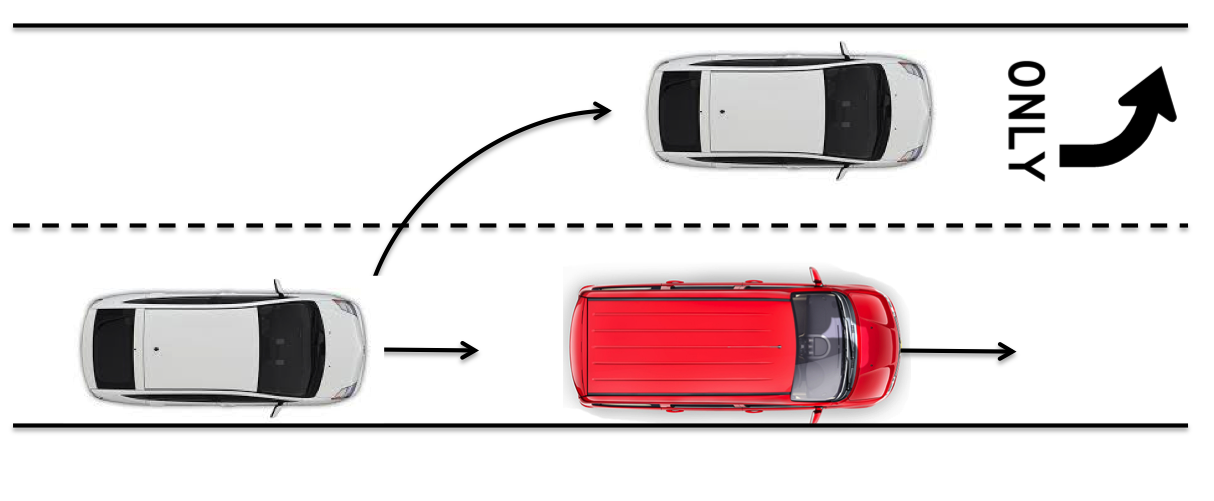
\includegraphics[scale=.4]{scenario.png}
	\caption{Pictorial description of ego vehicle's journey.}
	\label{fig:journey}
\end{figure}

The requirements are:
	\begin{enumerate}
		\item Velocity is always less than or equal to the speed limit
		\item Position is always at a minimum distance from other vehicles in the environment if in the same lane
		\item Eventually, drive a total length of 80m and end up in the left lane.
	\end{enumerate}

\subsection{Scenario 1: lane following}
The first scenario we identify in this journey is the Lane Following scenario. 
First we give the system model.
Both ego and other vehicles are modeled in the same manner. 
First we assume that there is no significant movement of the car along the direction perpendicular to the road's direction, \emph{as long as the vehicle is keeping to its lane}.
Thus the position is given by a scalar $s$.
Therefore, the state of a vehicle is 2-dimensional and given by its position $s$ along the road and velocity $v$: $x = (s,v)$.

A vehicle's dynamics are modeled using a Rectangular Hybrid Automaton: this is a class of hybrid systems where the continuous dynamics in each location are given by so-called rectangular inclusions, namely, $c_1 \leq \dot{x} \leq c_2$ for some rational constants $c_1$ and $c_2$. 
In our case, this means that the vehicles' dynamics are given by 
\[\left[\begin{matrix}
c_{s,1}\\c_{v,1}
\end{matrix}\right]
\leq
\left[\begin{matrix}
\dot{s}\\ \dot{v}
\end{matrix}\right]
\leq
\left[\begin{matrix}
c_{s,2}\\c_{v,2}
\end{matrix}\right]
\]

Thus the velocity $\dot{s}$ and acceleration $\dot{v}$ are bounded.
These are very general dynamics. 
In Section \ref{sec:relating-the-two-system-models} we see how we use this general form to over-approximate the behavior of the accurate nonlinear dynamics of the vehicles.

The elements of the Lane Following scenario are:
\begin{itemize}
	\item $A^1 = \{a\}$ is the set of other agents, in this case consisting of one other agent $a$ (red car in Fig. \ref{fig:journey}).
	\item $Road^1$ is a two-lane unidirectional road segment shown in Fig. \ref{fig:journey}.
	\item $Init^1 = X_{ego}^0 \times X_a$, where 
	$X_{ego} = [0,30] \times [0,1]$ and
	$X_a = [0,36] \times [0,1]$.
	That is, the initial position along the road is anywhere between 0 and 30 meters, and the initial velocity is between 0 and 1 m/s for the ego vehicle. 
	Analogously for the other vehicle.
	\item $\lawSet^1 = \{speedLimit, minSeparation\}$ where
	\[speedLimit \defeq \always (v_{ego} \leq v_{max})\]
	\[minSeparation \defeq \always (s_{ego} \leq s_a - 5)\]
	\item $\goal^1 = \eventually_{[0,30]}(s_{ego} \geq 80)$.
	That is, the ego vehicle must cover 80m in less than 30 seconds.
\end{itemize}

We verified this scenario using HyTech, a model checking tool for rectangular hybrid automata.
The HyTech tool returned the result in .01 seconds on a 32 bit Ubuntu machine on an 1.2 GHz Intel Opteron processor and 600 MB of RAM.

\subsection{Scenario 2: lane change}
The second scenario we identify is a Lane Change scenario.
When the car is performing such dynamic maneuvers with a real chance for safety violation, it is important to work with accurate dynamics, rather than simplified dynamics. 
In this scenario, we model the ego vehicle using a 7D bicycle model of a car, validated on a Cadillac SRX. 
The details of the model are given in the appendix.
We simply note here that the vehicle's position is given by the 2D variable $(s_x,s_y)$, where $s_x$ is the position of the vehicle in the horizontal direction (along the road) and $s_y$ is its position in the vertical direction (perpendicular to the road). 

The other vehicle, on the other hand, is modeled same as in the Lane Following scenario, using a differential inclusion. 
That is because we only care about knowing an envelope around where the other vehicle is.

The scenario elements are given by:
\begin{itemize}
	\item $A^2 = \{a\}$ is the set of other agents, in this case consisting of one other agent $a$ (red car in Fig. \ref{fig:journey}).
	\item $Road^2$ is a two-lane unidirectional road segment shown in Fig. \ref{fig:journey}.
	\item $Init^2 = X_{ego}^0 \times X_a$. 
	Here, $X_{ego}$ is a 7-dimensional subset of $\Re^7$.
	In particular, we consider that state variable $(s_x,s_y)$ starts at (0,0) without loss of generality. And 
	$X_a = [3,10] \times [0,1]$.
	\item $\lawSet^2 = \{speedLimit, minSeparation\}$ where
	\[speedLimit \defeq \always v_{ego} \leq v_{max}\]
	\[minSeparation \defeq \always s_{x,ego} \leq s_{x,a} - 3\]
	\item $\goal^2 = \eventually_{[0,7]}(s_{y,ego} = -W)$.
	That is, the ego vehicle must be in the left lane ($s_y = -W$ in our coordinate system) within 7s.
\end{itemize}

Because the dynamics are now nonlinear, we verify this scenario using dReach, a reachability analysis tool that can handle nonlinear dynamics.
Namely we ask dReach the question: can the system evolve in such a way that the ego vehicle violates its constraints or its goal? 
In this case, dReach returns a negative answer, thus estabilishing the formal correctness of the scenario.

\subsection{Scenario hand-off}
The correctness of the hand-off is established by verifying, using HyTech, that the first scenario either completes successfully (i.e. $\goal^1$ is satisfied), or the system evolves to a point where it satisfies the initialization $Init^2$ of the second scenario.

\subsection{Relating the two system models}
\label{sec:relating-the-two-system-models}
Because we want the two scenarios to be verified for the same underlying ego vehicle, it is important that the dynamics of the ego car in one scenario be an abstraction of its dynamics in the other scenario.
Alternatively, it suffices that they both be abstractions of the same underlying dynamics.
If model $M$ is an abstraction of model $N$, this means that all behaviors of $N$ can be exhibited by $M$. 
Then if $M$ is correct, we know a fortiori that $N$ is correct.

In our case, we over-approximated the nonlinear dynamics of the Lane Change scenario into the Rectangular Hybrid Automaton dynamics of the Lane Following scenario.
Thus we have a formal and verifiable relation between the two models.


\appendix
\section{Bike model of vehicle}
The nonlinear dynamics that we adopt as being the "ground truth" for the ego vehicle's movement are given by a 7D kinematic bicycle model.
The model considers that the two front wheels and two rear wheels of the vehicle move in unison, with steering provided by the front wheels only. 
Furthermore, each abstracted wheel is located along the center of the vehicles body and does not slip. 

Figure \ref{fig:bike} shows the state variables and parameters involved in the model.

\begin{figure}[t]
	\centering
	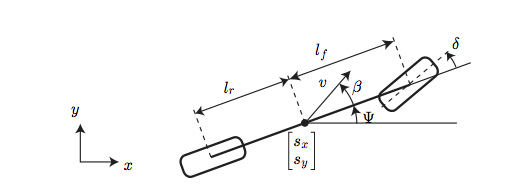
\includegraphics[scale=0.5]{figures/bicycle}
	\caption{Bicycle Model of the Ego Vehicle \cite{Althoff2014}}
	\label{fig:bike}
\end{figure}

\begin{table}[h]
	\label{table:vehiclep}
	\begin{tabular}{|c|c|c|c|c|c|}
		\hline
		\multicolumn{6}{|c|}{Vehicle Parameters} \\ \hline
		\textit{$m$} & \textit{$I_z$} & \textit{$C_f$} & \textit{$C_r$} & \textit{$l_f$} & \textit{$l_r$} \\ \hline
		2273 kg & 4423 kg*m$^2$ & 10.8e4 N/rad & 10.8e4 N/rad & 1.292 m & 1.515 m \\ \hline
	\end{tabular}
	\caption{Parameters of Example Ego Vehicle}
\end{table}

The parameters \(C_f,C_r\) and \(l_f, l_r\) describe respectively the cornering stiffness and distances from the center of gravity to the axles respectively. The moment of inertia, \(I_z\) and the vehicle mass, \(m\) are experimentally determined constants \cite{Snider2009}. 
The parameters of the model can be experimentally determined and validated.
Their values for the Cadillac SRX model, as reported by \cite{Althoff2014}, are shown in Table \ref{table:vehiclep}.

The variable \(\beta\) is the slip angle at the center of mass, \(\psi\) is the heading angle, \(\dot{\psi}\) is the yaw rate, \(v\) is the velocity, \(s_x\) and \(s_y\) are the x and y positions, and \(\delta\) is the angle of the front wheel. 
In the formulation of \cite{Althoff2014}, the inputs to the system are \(a_x\), the longitudinal acceleration, and \(v_w\) the rotational speed of the steering angle. The \(y\) terms represent disturbances to the system. 
For example \(y_{\beta}\) and \(y_{\dot{\psi}}\) represent disturbances to the slip angle at the center of mass and the yaw rate. The state equations for the system are:
\begin{gather*}
\label{eqn:beta}
\dot{\beta}=\left(\frac{C_rl_r-C_fl_f}{mv^2} \right)\dot{\psi}+\left(\frac{C_f}{mv} \right)\delta-\left(\frac{C_f+C_r}{mv} \right)\beta+y_{\beta}
\\
\label{eqn:psi}
\ddot{\psi}=\left(\frac{C_rl_r-C_fl_f}{I_z} \right)\beta-\left(\frac{C_fl_f^2-C_rl_r^2}{I_z} \right)\left(\frac{\dot{\psi}}{v} \right)+\left(\frac{C_fl_f}{I_z} \right)\delta+y_{\dot{\psi}}
\\
\label{eqn:v}
\dot{v}=a_x+y_v
\\
\label{eqn:sx}
\dot{s_x}=v\cos{(\beta+\psi)}+y_{s_x}
\\
\label{eqn:sy}
\dot{s_y}=v\sin{(\beta+\psi)}+y_{s_y}
\\
\label{eqn:delta}
\dot{\delta}=v_w+y_d
\end{gather*}


\subsection{Tracking Controller}
The scenario model considers a simple path tracking controller which was successfully implemented and used on the CMU DARPA Grand Challenge vehicle. Path tracking controllers guide a vehicle along a geometrically defined trajectory by apply steering and longitudinal acceleration inputs. A successful path tracking algorithm maintains vehicle stability and attempts to minimize the error between the desired trajectory and actual trajectory. The parameters computed for this controller when implemented and validated on a Cadillac SRX \cite{Althoff2014}.

Thus, the feedback to the system are the lateral and longitudinal tracking errors. We derive the following results as in  \cite{Snider2009}:
\begin{gather*}
\epsilon_x=cos{(\Psi_d)}(s_{x,d}-s_x) +sin{(\Psi_d)}(s_{y,d}-s_y)
\\
\epsilon_y=-sin{(\Psi_d)}(s_{x,q}-s_x)+cos{(\Psi_d)}(s_{y,d}-s_y)
\end{gather*}
Through the lateral tracking error, and desired trajectory we can then compute the desired rate of change of the angle of the front wheel with respect to time. This enables the computation of rate of change of the rotational speed of the steering angle. We note that the relevant parameters are again defined using the validated model in \cite{Althoff2014}.
\begin{gather*}
\delta_d=k_1 \epsilon_y+k_2(\Psi_d-\Psi)+ k_3(\dot{\Psi_d}-\dot{\Psi})
\\
v_w=k_4(\delta_d-\delta)
\end{gather*}
The longitudinal acceleration is simply defined by the tracking error between the actual velocity and the desired velocity.
\begin{gather*}
a_x=k_5\epsilon_x+k_6(v_d-v)
\end{gather*}
Combining the equations as in \cite{Althoff2014} the control inputs for longitudinal acceleration (pressing the accelerator) and steering angle velocity (turning the steering wheel) can be computed as $v_w$ and $a_x$ respectively. 
\begin{gather*}
v_w=k_1(cos{(\Psi_d)}(s_{y,d}-s_y-w_y)-sin{(\Psi_d)}(s_{x,d}-s_x-w_x))+k_2(\Psi_d-\Psi-w_{\Psi})\\ +k_3(\dot{\Psi_d}-\dot{\Psi}-w_{\psi})-k_4(\delta-w_{\delta})
\\
a_x=k_5(cos{(\Psi_d)}(s_{x,d}-s_x-w_x)+sin{(\Psi_d)}(s_{y,d}-s_y-w_y))+k_6(v_d-v-w_v)
\end{gather*}

\subsection{Trajectories}
To use the tracking controller in the lane change scenario, we must specify a lane change trajectory for the controller to track.
In our simple example, we use a simple hyperbola $s_{x,d} = s_{y,d}^3$ with inflection point at the current position of the car.
By substituting this into the equations above we obtain $\Psi_d$, and the closed-loop dynamics of the system. 
Other trajectories can be used and the analysis that follows is unchanged.
%In order to define a valid trajectory and controller for a lane change maneuver several constants beyond the controller parameters must be specified.
%We state that $w$ is the width of the road in meters and $v_d$ is the desired velocity of the vehicle in $m/s$. 
%We also define variable $t$ to represent time is units of seconds. 
%We then define the quantity $v_{mag}$ which is the magnitude of the vehicle's velocity vector measured in $m/s$.
%For convenience, we compute the magnitude of the velocity vector at time $t$.
%\begin{gather*}
%v_{mag}=\sqrt{9(t-.5w)^4 +1}
%\end{gather*}
%
%The individual quantities of $\dot{s_{x_d}}$ and $\dot{s_{y_d}}$ are as follows:
%\begin{gather*}
%\dot{s_{x_d}}=3v_d(t-.5w)^2/v_{mag}\\
%\dot{s_{y_d}}=v_d/v_{mag}\\
%\end{gather*}
%
%Finally the first and second derivative of the steering angle are:
%\begin{gather*}
%\dot{\Psi_d}=(48w-96t)/(81*(w-2t)^8)\\
%\ddot{\Psi_d}=96(-16+27(-2t+w)^4)/(16+9(-2t+w)^4)^2
%\end{gather*}



\bibliographystyle{abbrv}
\bibliography{emsoft15,mok}



\end{document}